\documentclass[11pt, a4paper]{article}
\usepackage[utf8]{inputenc}
\usepackage[left=2cm, right=2cm, top=2.5cm, bottom=2.0cm]{geometry}
\usepackage{amsmath, amssymb, amsthm}
\usepackage[english]{babel}
\usepackage{graphicx}
\usepackage[font={small,it}]{caption}
\graphicspath{ {figures/} }
\usepackage{url}
\usepackage{appendix}
\usepackage{float}
\usepackage{multirow}
\usepackage[bottom]{footmisc}
\usepackage{wrapfig}
\usepackage{subcaption}
\usepackage{titling}
\setlength{\droptitle}{-10em}  

\title{ \huge Artificial neural networks \\ 
  { \large Assigment 3: Recurrent neural networks }}
\author{
        Lood, Cédric \\
        \small Master of Bioinformatics
}

\begin{document}
\maketitle

\section{Context}
In this exercise, we explore the use of recurrent neural networks and
their applications as associative memories. Items can be stored as
equilibrium points of the network, similarly to those in dynamical
systems.

\section{Hopfield network}

In this section, we use hopfield neural networks to store 10 digitized
handwritten digits. The network has an architecture of 240 neurons,
fully connected and arranged in a single layer, with a saturation
function \emph{satlins}. It is trained in such a way that each digit
is an attractor point of the network, where they represent minimums of
the energy function. To note is that with an architecture consisting
of 240 neurons, the storage of 10 patterns is possible with a small
chance of error.

The first column of the left-hand side of figure \ref{fig:ndigits1}
corresponds to the patterns that are stored in the network. Each digit
is encoded as a 15 by 16 vector of pixels. Each 3 pairs of columns
following the digits in the first column corresponds to an attempt at
retrieving a noisy digit (the first column in a pair) through a fixed
amount of iterations. As can be seen, the process is fairly good,
failing only when the amount of noise is large - examples of failures
are located in the last column of the digits 2, incorrectly
reconstructed as a 7, and the digit 9, incorrectly reconstructed as a
2. In both cases, the error do seem to make sense to the human
eye. What happens there is that we jump from the neighborhood of the
correct attractor due to the noise to the neighborhood of another
attractor.

Similarly, the first column of the figure \ref{fig:ndigits2} displays
the original pattern. A fixed amount of noise is then introduced (2.5
in our example), then an iterative reconstruction process is
attempted.

\begin{figure}[H]
    \centering
    \begin{subfigure}{.5\textwidth}
      \centering
      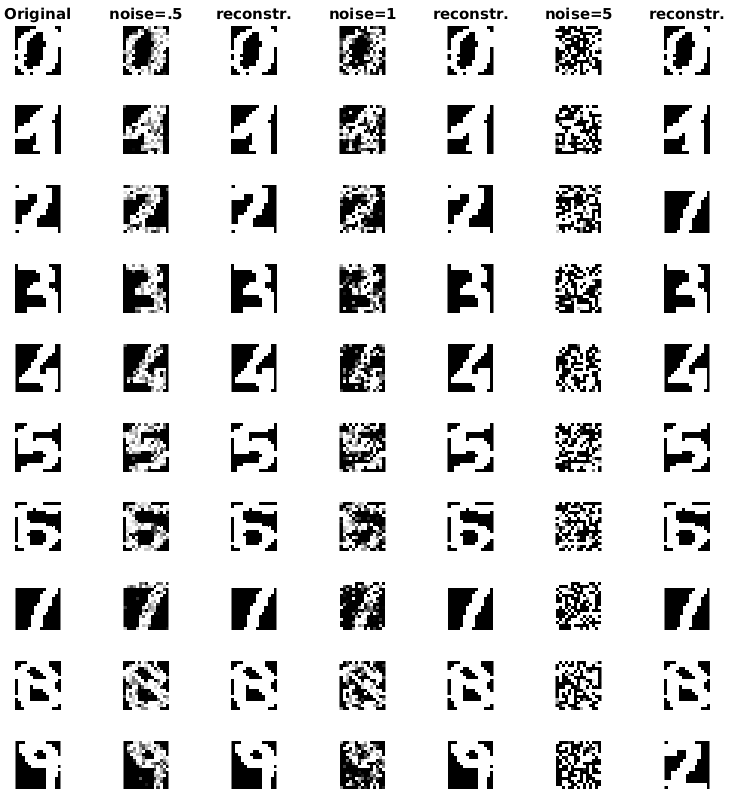
\includegraphics[width=0.90\linewidth]{ndigits_fi1.png}
      \caption{Fixed amount of iterations (50)}
      \label{fig:ndigits1}
    \end{subfigure}%
    \begin{subfigure}{.5\textwidth}
      \centering
      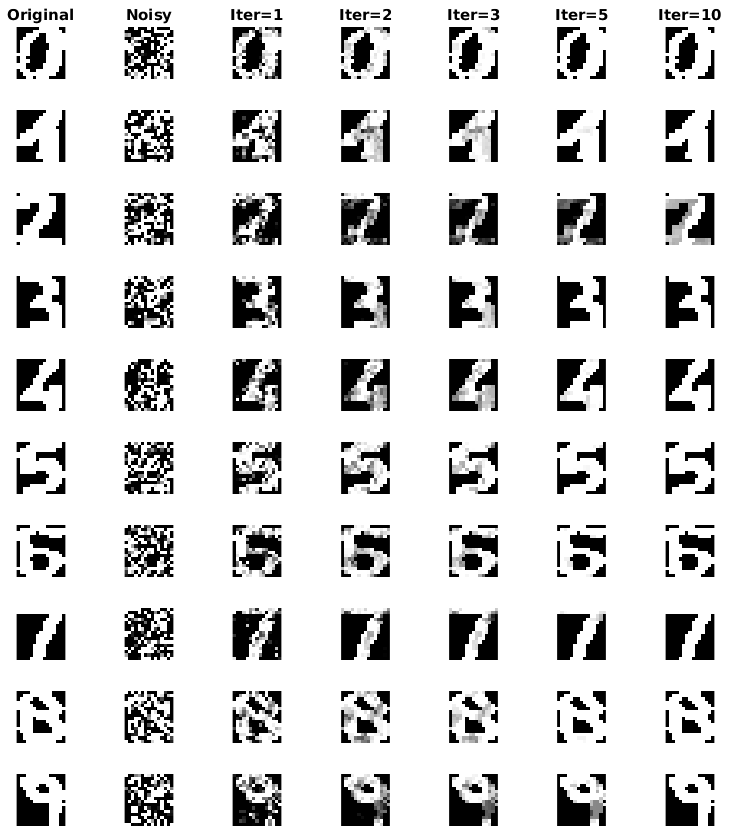
\includegraphics[width=0.85\linewidth]{ndigits_fn2.png}
      \caption{Fixed amount of noise (2.5)}
      \label{fig:ndigits2}
    \end{subfigure}
    \caption{Hopfield network reconstruction of noisy digits}
    \label{fig:ndigit}
\end{figure}

I did not detect spurious states - which are attractors not put in
explicitely in the network. The probability that some exists though is
not null.

\section{Elman network}

In this section, I investigated the use of Elman recurrent networks,
known to be able to deal with time varying patterns, on a so-called
\emph{Hammerstein system}. Elman network consists in two-layers, a
hidden one, that uses sigmoid transfer function and has a feedback to
the input, and an output layer that uses a linear transfer function.

To determine appropriate numbers of epochs to use and the number of
hidden neurons for the network, I investigated systematically multiple
settings and looked at the test MSE.

\bibliographystyle{ieeetr} 
\bibliography{bib-db}


\end{document}
